\documentclass[letterpaper,twocolumn,10pt]{article}
\usepackage{usenix,epsfig,endnotes}
\usepackage{graphicx}
\usepackage[labelfont=bf]{caption}
\usepackage{amsmath}
\usepackage{stfloats}

\setlength\parindent{0pt}

\begin{document}

%don't want date printed
\date{}

%make title bold and 14 pt font (Latex default is non-bold, 16 pt)
\title{\Large \bf ECE 225A Project Report - California Housing Prices Prediction}

\author{
{\rm Kirtan Shah}\\
Department of Electrical and Computer Engineering, University of California, San Diego
}

\maketitle

% Use the following at camera-ready time to suppress page numbers.
% Comment it out when you first submit the paper for review.
\thispagestyle{empty}


\subsection*{Abstract}

This project analyzes California Housing Prices and predicts median house values using Linear Regression, K Nearest Neighbors, Random Forest, and XGBoost. 

\section{Introduction}
The California housing market has long been a subject of interest for economists, policymakers, and residents. 
This paper presents an exploratory data analysis of the California Housing Prices dataset, a collection of housing-related statistics from the 1990 California census \cite{kaggleCaliforniaHousing}.
For this project, I focus on uncovering insights into patterns within the data, especially in relation to median house values across different census blocks in California. 
Through data preprocessing, statistical modeling, and visualization techniques, I explore features and their predictive value in determining median house values.
I also compare regression models for median house values, which provide further insight into the complex dynamics of California's housing market.


\section{Dataset}
The California Housing Prices dataset \cite{kaggleCaliforniaHousing}, provided by the US Census and available on Kaggle, comprises housing-related statistics for different blocks in California.
Each entry represents statistics for a group of homes in a given block.

\subsection{Dataset Description}
These variables include the following:
\begin{itemize}
    \item Latitude and longitude
    \item Median house age within block
    \item Total rooms, total bedrooms
    \item Total population
    \item Number of households in block
    \item Median income for households in block
    \item Median house value for households in block
    \item Ocean proximity (<1H OCEAN, INLAND, ISLAND, NEAR BAY, NEAR OCEAN)
\end{itemize}

% figure for image
\begin{figure}%[h]
\centering
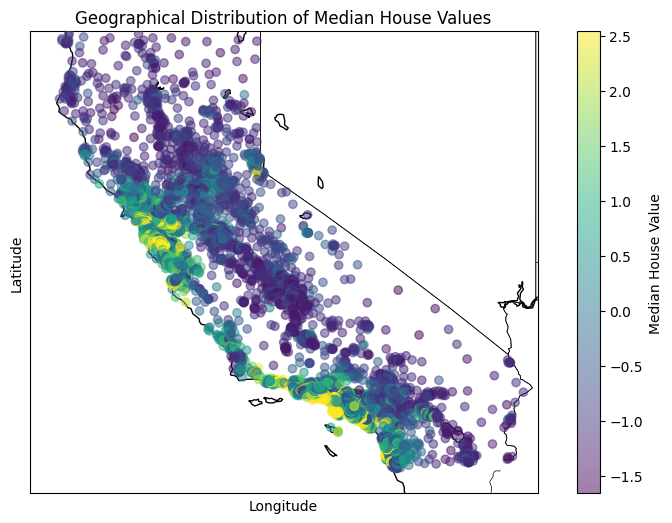
\includegraphics[width=0.5\textwidth]{images/california_map.png}
\caption{Visualization of California median house values}
\label{fig:california_map}
\end{figure}

The dataset contains 20640 entries corresponding to a different census block, each with the features described above.

\subsection{Exploratory Data Analysis}

The dataset contains a variety of numerical and categorical features, wich need proper preprocessing before they can be used for analysis.
First, we recognize the categorical variable of ocean proximity, for which it would make little sense to represent numerically; for example, if ISLAND is mapped to 1 and NEAR OCEAN is mapped to 2, it implies that NEAR OCEAN is somehow twice whatever ISLAND represents, which doesn't necessarily make sense.
Thus, we use one-hot encoding to represent the ocean proximity variable as a set of binary variables, each representing a different category.
Here is an example one hot vector for an entry with ISLAND:

\begin{equation}
    V_{\text{ISLAND}} = \begin{array}{c}
        \text{<1H OCEAN} \\
        \text{INLAND} \\
        \text{ISLAND} \\
        \text{NEAR BAY} \\
        \text{NEAR OCEAN}
    \end{array}
    \begin{bmatrix}
        0 \\
        0 \\
        1 \\
        0 \\
        0
    \end{bmatrix}
\end{equation}

Next, we normalize the numerical features to ensure that they are on similar scales and have relatively small values.
This is important because we don't want to bias metrics like correlation or our predictor towards features with larger values (e.g. latitude/longitude) over those with smaller values (e.g. total rooms).
Therefore, we normalize each feature to have a mean of 0 and a standard deviation of 1 as follows:

\begin{equation}
    x' = \frac{x - \mu}{\sigma}
\end{equation}

With the preprocessed features, we can now analyze the data to uncover patterns and relationships between different features.
One way to do this is by computing the correlation matrix for the features, which gives us a sense of how each feature is related to the others.
This is done by computing a matrix \(C\) where \(C_{ij}\) is defined in equation~\ref{eq:corr_matrix}.
\begin{equation}
    C_{ij} = \frac{Cov(X_i, X_j)}{\sigma_i \sigma_j} 
    \label{eq:corr_matrix}
\end{equation}

\begin{figure}%[h]
    \centering
    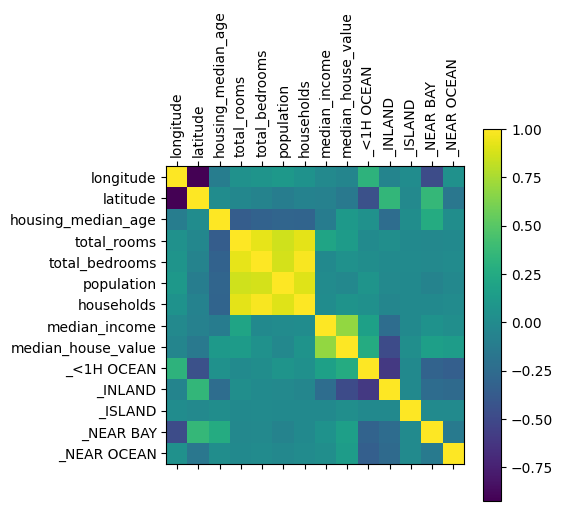
\includegraphics[width=0.5\textwidth]{images/corr_matrix.png}
    \caption{Correlation matrix for housing features}
    \label{fig:correlation_matrix}
\end{figure}

The correlation matrix is visualized in Figure~\ref{fig:correlation_matrix}. Notice that similar features like total rooms and total bedrooms have a high correlation, while features relating to ocean proximity have low correlation with population and number of households.
Most importantly, the median house value has the highest correlation with median income, which suggests that income could be key factor in determining house prices.


Zooming into median house value correlations specifically, we plot the magnitudes of the correlations of each feature and median house value in Figure~\ref{fig:correlation_mhv}.
From correlations alone, it seems that median income and ocean proximity seem to be the most important features in determining median house value.
\begin{figure}
    \centering
    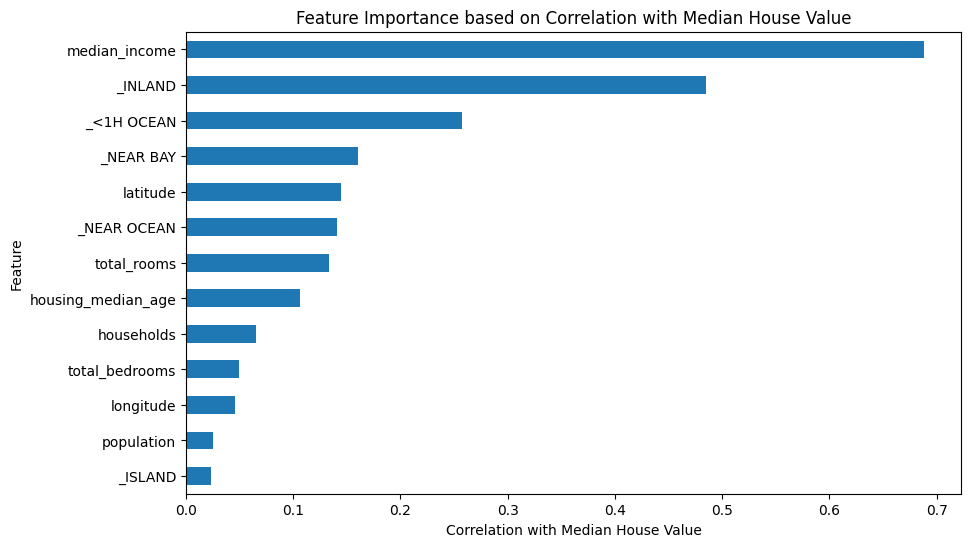
\includegraphics[width=0.5\textwidth]{images/feature_import_corr.png}
    \caption{Inferred Feature Importance based on correlation with median house value}
    \label{fig:correlation_mhv}
\end{figure}

\begin{figure}%[h]
    \centering
    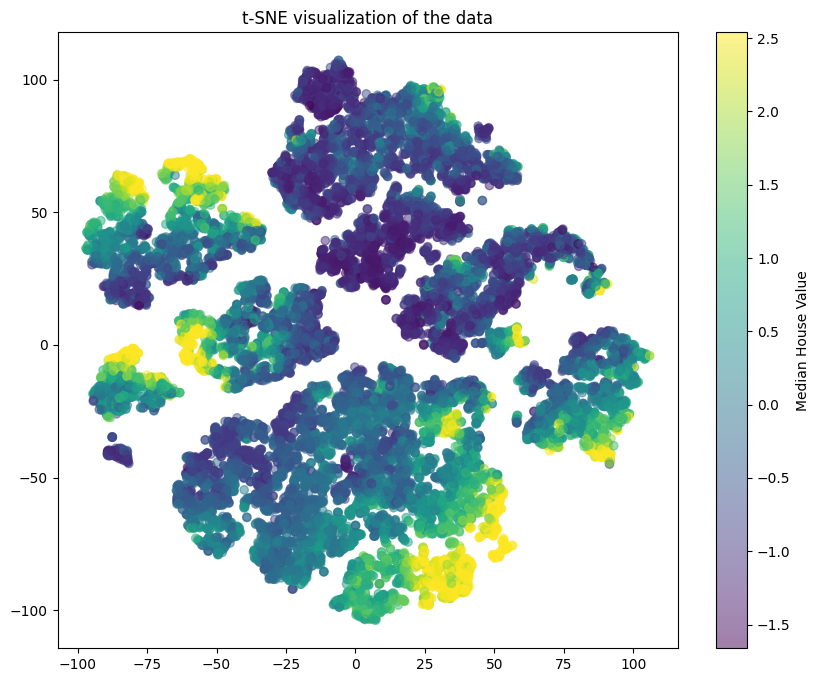
\includegraphics[width=0.5\textwidth]{images/tsne.png}
    \caption{t-SNE visualization of California housing data}
    \label{fig:tsne}
\end{figure}

With 20640 rows of multi dimensional data, it is hard to visualize the complexity (or hidden simplicity) of the data in a condensed plot.
However, a technique called t-SNE (t-distributed stochastic neighbor embedding) can be used to reduce the dimensionality of the data to 2D for visualization purposes \cite{tsne}. 
Figure~\ref{fig:tsne} shows the t-SNE visualization of the California housing data, and reveals the presence of several clusters of data points. This suggests that an algorithm like K-Nearest Neighbors, which relies on values of proximal data points, could be effective in predicting median house values.

\section{Predictive Modeling}
\begin{figure*}
    \centering
    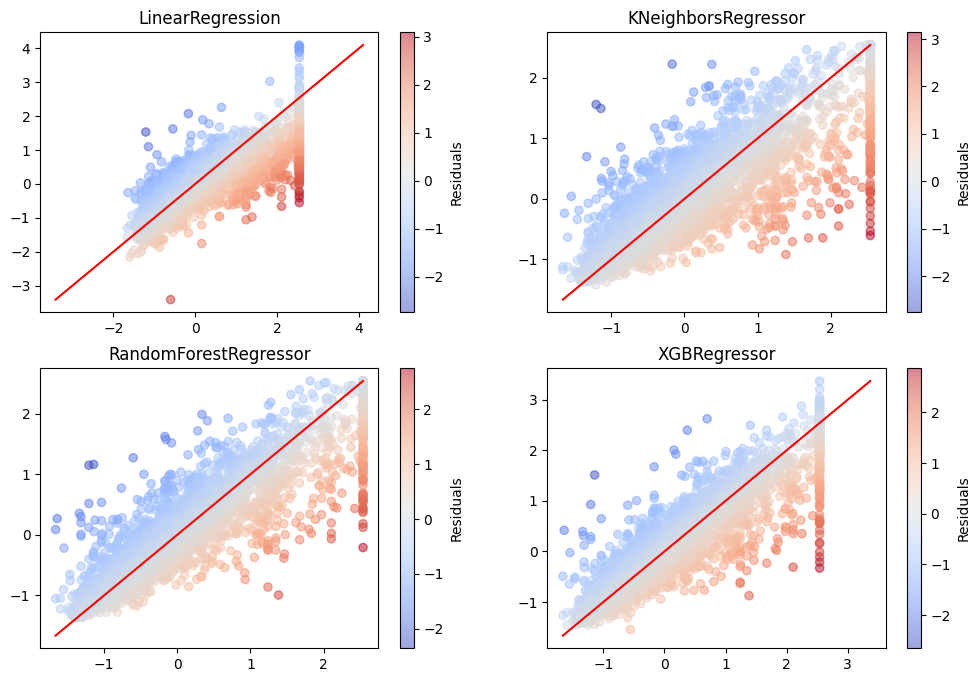
\includegraphics[width=.8\textwidth]{images/results.png}
    \caption{Predicted vs Actual Median House Values}
    \label{fig:results}
\end{figure*}

In this section, we will explore the use of a few different regression models to predict median house values based on the features in the dataset.

\subsection{Models}
We will start off with a Linear Regression model.
Based on the findings from the exploratory data analysis, we will try to improve results with a K Nearest Neighbors regressor. Finally, we utilize a Random Forest regressor and XGBoost regressor to see if we can further improve our predictions with state-of-the-art, popular models.

\subsection{Evaluation}
In order to accurately evaluate the performance of each model, we split the data into a training set and a test set.
For this project, we use a split of 80\% training data and 20\% test data.
The evaluation metric is the mean squared error (MSE), which measures the average squared difference between the predicted and actual median house values.
A lower MSE indicates a better model.

\begin{equation}
    MSE = \frac{1}{n} \sum_{i=1}^{n} (y_i - \hat{y}_i)^2
\end{equation}



\section{Results}

The models are evaluated based on their mean squared error (MSE) on the test set.
The results are summarized in Table~\ref{tab:results}.

\begin{table}[h]
    \centering
    \begin{tabular}{|c|c|}
        \hline
        Model & MSE \\
        \hline
        Linear Regression & 0.3624 \\
        K Nearest Neighbors & 0.2884 \\
        Random Forest & 0.1838 \\
        XGBoost & 0.1741 \\
        \hline
    \end{tabular}
    \caption{Model Performance}
    \label{tab:results}
\end{table}

For a more holistic view of the model performance, we plot the predicted vs actual median house values for each model in Figure~\ref{fig:results}.
The hypothesis that median house values tend to be clusters seems to be somewhat correct, with K Nearest Neighbors performing better than Linear Regression.
Yet, Random Forest and XGBoost regressors perform the best, with XGBoost having the lowest MSE of 0.1741.
Random Forest is an ensemble model that uses multiple decision trees to make predictions \cite{randomforest}, while XGBoost is a gradient boosting model combined with decision trees \cite{xgboost}.
The superior performance of these models suggests that the relationships between the features and median house values are complex and non-linear. 
Interestingly, features like ocean proximity and median income continue to be important in the XGBoost, corroborating what we found with the correlation matrix.
I conclude that the top most features in Figure~\ref{fig:xgboost_import} are the most important in determining house value.

\begin{figure}
    \centering
    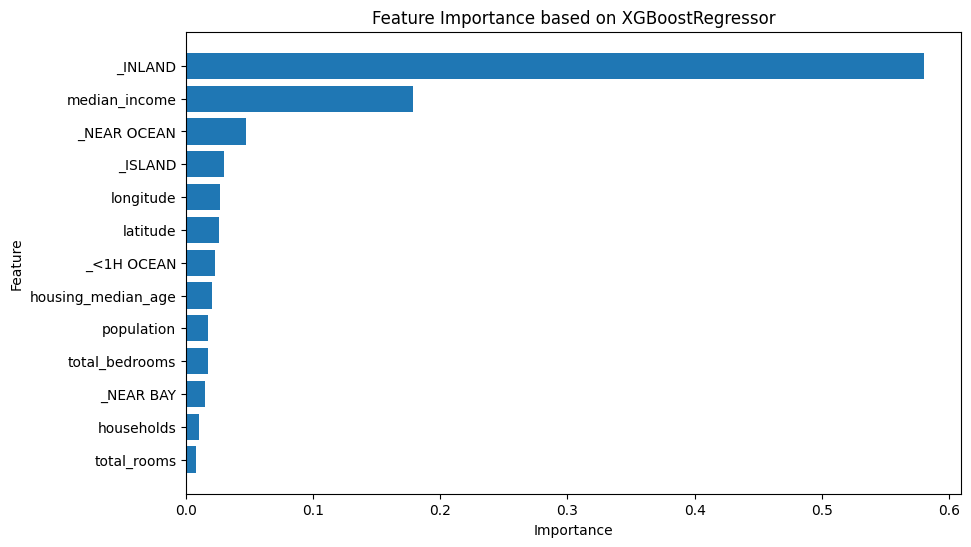
\includegraphics[width=0.5\textwidth]{images/feature_import_xgb.png}
    \caption{Feature Importance in XGBoost Model}
    \label{fig:xgboost_import}
\end{figure}

\section{Conclusion}
In this project, I conducted an exploratory data analysis of the California Housing Prices dataset, focusing on uncovering patterns and relationships between different features.
I found that median income and ocean proximity are the most important features in determining median house values, specifically whether or not a home is inland.


\section{Code}
\begin{flushleft}
The code for this project is uploaded to GitHub at \url{https://github.com/kirtan-shah/ECE225A-California-Housing-EDA}.
\end{flushleft}

{\footnotesize \bibliographystyle{acm}
\bibliography{sample}}


\end{document}







